\documentclass[12pt, a4paper, twoside]{article}
\usepackage[utf8]{inputenc}
\usepackage[cm]{fullpage}
\usepackage{fancyhdr}
\usepackage{textcomp}
\usepackage{graphicx}

\begin{document}

\title{Relatório do Experimento 3 de OAC}
\author{
Arthur Bizzi: 13/0102636 \\
Arthur da Silveira Couto: 16/0002575 \\
Caio Albuquerque Brandão: 16/0003636 \\
Cristiano Silva Júnior: 13/0070629 \\
Leonardo Maffei: 16/0033811 \\}
\date{X de Junho de 2017}
\maketitle

\section{Exercício 1}

\subsection{Exercício 1.1}

\subsection{Exercício 1.2}


% Como adicionar uma figura
% \begin{figure}
%     \centering
%     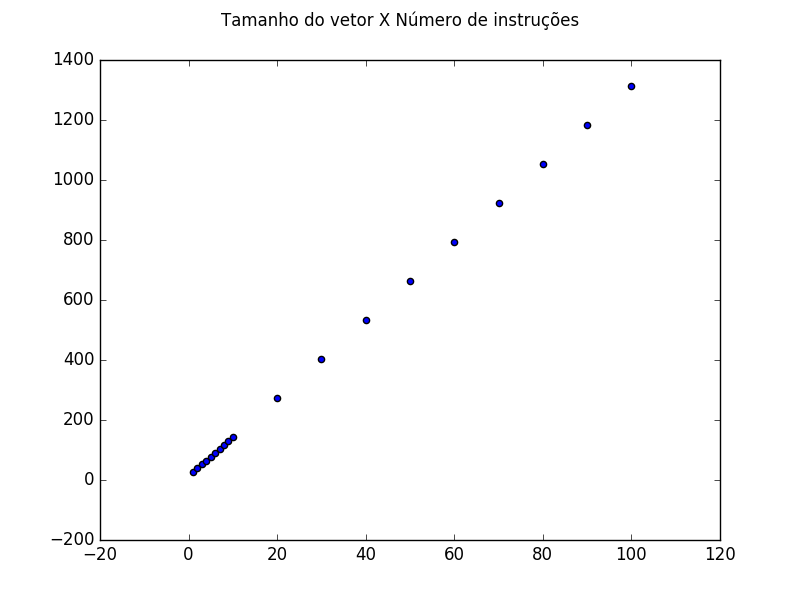
\includegraphics[width=0.8\textwidth]{ex1/best.png}
%     \caption{Melhores casos de ordenamento}
% \end{figure}



\section{Exercício 2}

% TODO Fazer questão 2 do relatório


\end{document}
